\chapter{Neural Networks}
\label{fundamentals:neural_network}

Neural networks, in the following referred to as NN, are a model used in the area of machine learning, which is biologically motivated and loosely mimics the function of the human brain. In the following paragraphs, we're going to explain the functions of all the components which make up a NN.

\paragraph{Neuron}\label{basic:neural_network:neuron} A NN, at the lowest level, is composed by \emph{neurons}, sometimes also called \emph{perceptrons}. These neurons are basically modelling a mathematical functions and are the building blocks of every NN.

These neurons accept $n$ input values $\mathbf{x} = (x_0, x_1, \dots, x_n)$ and use them to compute a single output value $o$. A unique weight $w_n$ from the set $\mathbf{w} = \{w_0, w_1, \dots, w_n\}$ is assigned to each of the input values. The input value of $x_0$ is almost always set to $1$ and not further changed; this value is the called the \emph{bias} value and allows the modelled function to affine instead of linear. This increases the modelling power of such neurons, as the space of functions which can possibly be modelled grows. With the aforementioned input values $\mathbf{x}$, the associated weights $\mathbf{w}$ and the activation function $\varphi$, the output $o$ of the neuron can be computed as shown in equation \ref{fundamentals:neural_network:compute_equation}:

\begin{equation}
o = \varphi(\mathbf{w} \cdot \mathbf{x}) = \varphi\bigg(\sum_{i=0}^{n} w_i x_i\bigg)
\label{fundamentals:neural_network:compute_equation}
\end{equation}

The activation function $\varphi$ is responsible for squeezing the result of the computation of a neuron into a predefined range of values; for example using \emph{tanh} always results in output values in the range $[-1, +1]$, no matter which scale the input values originally had. Examples of commonly used activation functions are \emph{tanh}, \emph{relu}, \emph{sigmoid} or \emph{binarystep}. They are visualized as plots in figure \ref{fundamentals:figures:activation_functions}.

\begin{figure}[h]
	\subfigure[$\tanh(x) = \frac{e^x - e^{-x}}{e^x + e^{-x}}$]{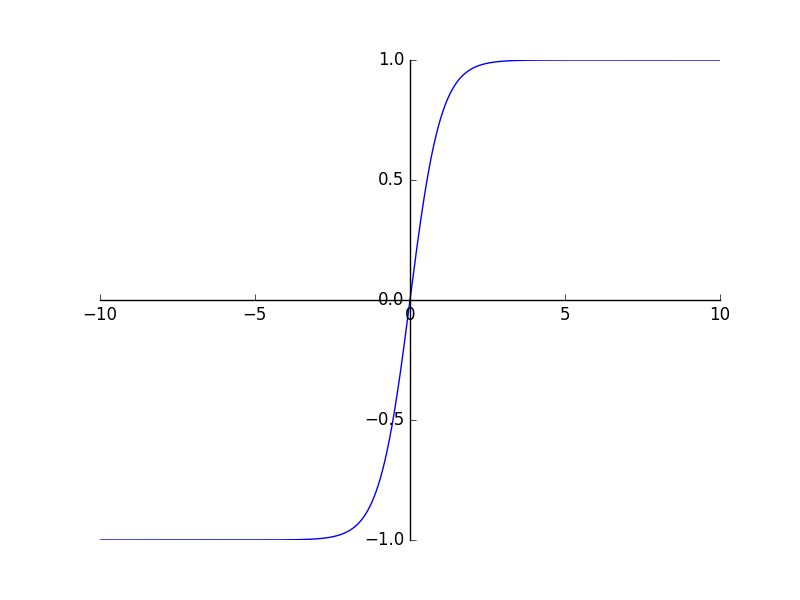
\includegraphics[width = 3in]{img/tanh_activation}}
	\subfigure[$\operatorname{sigmoid}(x) = \frac{1}{1 + e^{-x}}$]{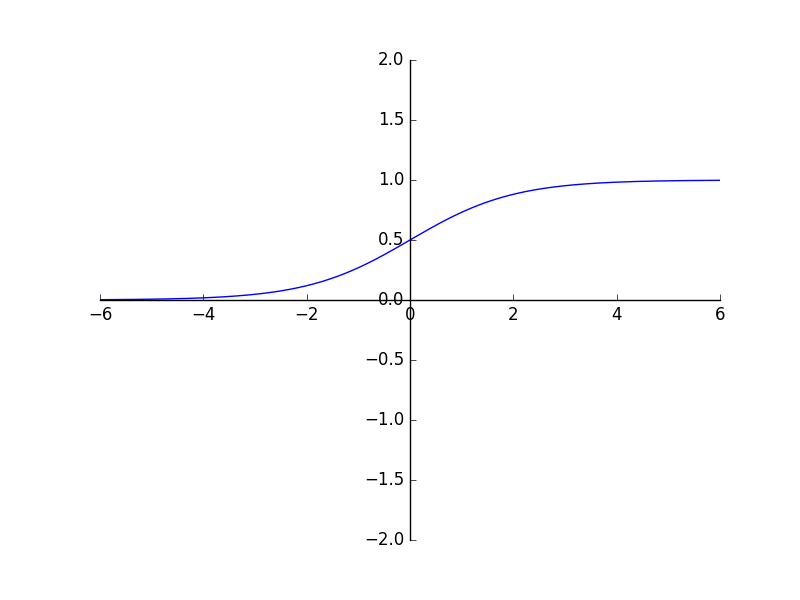
\includegraphics[width = 3in]{img/sigmoid_activation}}
	\subfigure[$\operatorname{relu}(x) = \max\{0,x\}$]{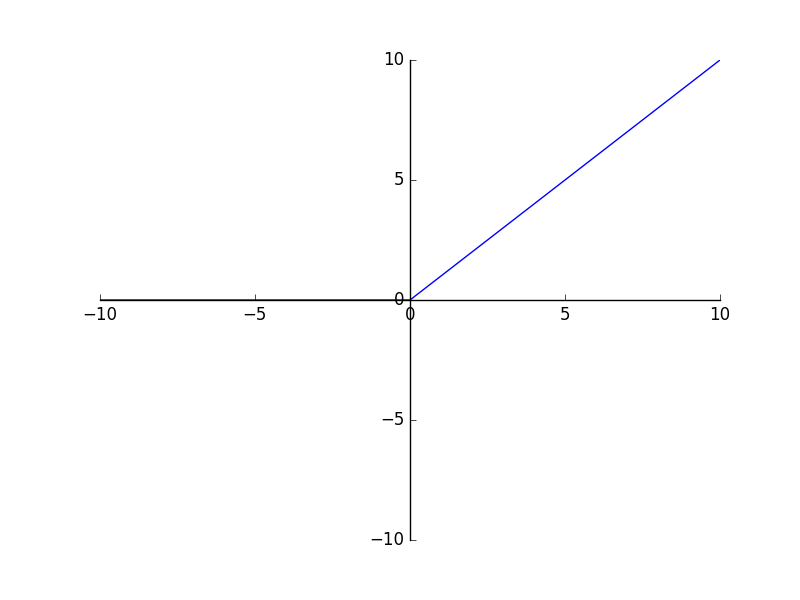
\includegraphics[width = 3in]{img/relu_activation}}
	\subfigure[][{$\operatorname{binarystep}(x) = \left\{\begin{array}{lr}0 & \text{for }x < 0\\1 & \text{for }x \geq 0\end{array}\right\}$}]{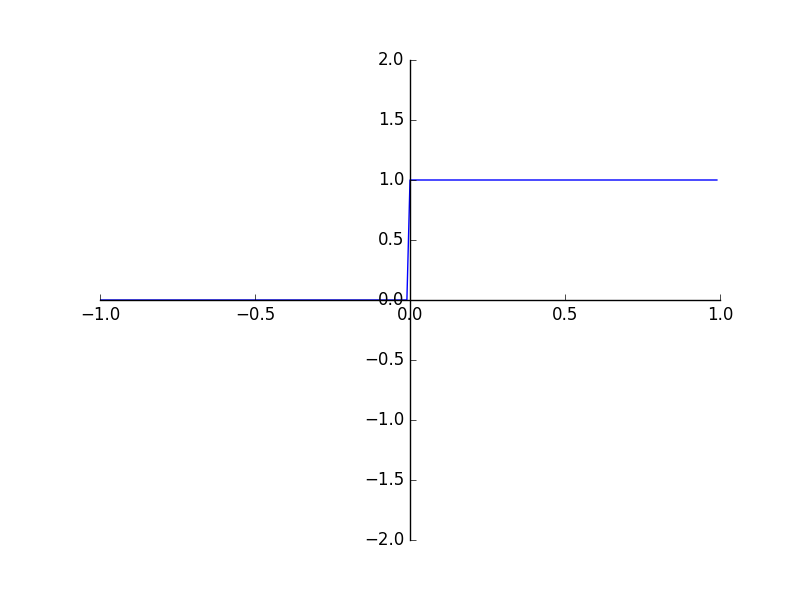
\includegraphics[width = 3in]{img/binary_step_activation}}
	\caption{Plots of several commonly used activation functions for neurons in NNs.}
	\label{fundamentals:nn:figures:activation_functions}
\end{figure}

\paragraph{Layer}\label{basic:neural_network:layer} With the neurons introduced one paragraph earlier, we can now start to build the layers of a NN. Each layer consists of multiple neurons stacked on top of each other, as seen in figure \ref{fundamentals:figures:neural_network}. These layers are then arranged in a sequential manner to form a full NN. Each NN usually has at least three of these layers: The first one is called the \emph{input layer}, the second the \emph{hidden layer} and the most right one is the \emph{output layer}.

\begin{figure}[h]
	\centering
	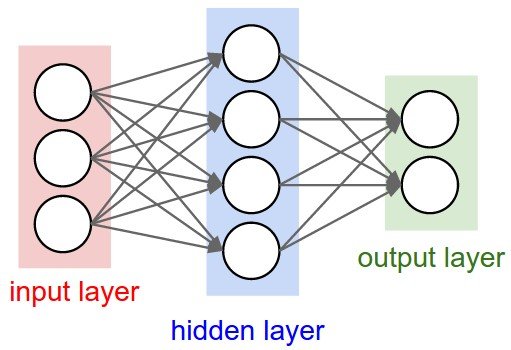
\includegraphics[width=10cm]{img/basic_neural_network}
	\caption{Simplified visualization of a NN with one input, hidden and output layer.}
	\label{fundamentals:figures:neural_network}
\end{figure}

The input data $\mathbf{x} = (x_1, x_2, \dots, x_n)$ is enters the NN through the input layer. At this stage, the bias $x_0$ value is usually set to $1$ again. Most of the time, there is only one bias value and weight for all neurons in a layer of an NN. The input values in $\mathbf{x}$ are then forwarded to the neurons of the (first) hidden layer which then compute their activations $o_{ln}$, where $l$ signifies the layer and $n$ shows the position of the neuron in that layer respectively. The resulting activation values are then passed to the output layer, where the embodied neurons compute their activation values $o_{21}, o_{22}, \dots, o_{2n}$. The input values of a single neuron in the output layer are usually the activation values of all neurons in the preceding layer. Such a layer is also called \emph{fully-connected}, as every neuron uses all values from the preceding layer. The output of the NN is then the set of activation values $o_{31}, o_{32}, \dots, o_{3m}$ in the output layer, where $m$ signifies the number of neurons in the output layer.

This procedure of doing one forward-pass through the NN is called \emph{forward propagation}. Our example only consists of one hidden layer, but one can also imagine NNs with multiple hidden layers; such NNs are then called \emph{deep neural networks}. The number of layers and neurons in each of them is strongly dependent on the nature of the problem it is applied to.

\paragraph{Backpropagation with gradient-descent} As in almost all models in the area of machine learning, a NN learns by optimizing a \emph{loss function} $L$, also sometimes called error function. Every function which can be used to quantify the predictive error of a NN can be used as a loss function. As examples, one could mention the \emph{mean squared deviation} $\operatorname{msd}(y_{true}, y_{pred}) = \frac{1}{n}\sum_{i=0}^{n} (y_{pred} - y_{true})^2$ or the one used for the model of this thesis, the \emph{categorical cross-entropy} function $H(p,q) = -\sum{x} p(x)\operatorname{log}(q(x))$. The optimization of this loss function is almost always done via a method called \emph{backpropagation} in conjunction with the \emph{gradient-descent} algorithm. The optimization is then done as follows:

\begin{enumerate}
	\item Do the forward propagation with the given input values $\mathbf{x} = (x_0, x_1, \dots, x_n)$ as described above.
	\item Use the predicted and expected values in combination with the defined loss function to quanitfy the predictive error of the NN.
	\item The predictive error is now backpropagated through the NN via the gradient-descent algorithm. The weights of all inputs for each neuron are then adapted with respect to their influence on the exhibited predictive error.
\end{enumerate}

The influence of each weight on the predictive error is determined by computing the partial derivate of the loss function $L$ with respect to the respective weights, as seen in equation \ref{fundamentals:equation:gradient_descent}. After computing the partial derivation, the weights are updated accordingly. This is done by multiplying the computed derivation value by the learning rate $\eta$ and subtracting the resulting value from the current value of the weight. The learning rate defines, how strong a single run of gradient-descent alters each weight in the network.

The new value for the weight $i$ in layer $l$, with given learning rate $\eta$ and loss function $L$, is then computed as follows:

\begin{equation}
\label{fundamentals:equation:gradient_descent}
w_{li} \coloneqq w_{li} - \eta \frac{\delta E(\mathbf{w})}{\delta w_{li}}
\end{equation}

In practice, this computation is done in a vectorized manner to speed up the computation significantly. Here we use the gradient (hence the name) of the loss function with respect to all weights $\mathbf{w}$:

\begin{equation}
\mathbf{w} \coloneqq \mathbf{w} - \eta(\nabla_{\mathbf{w}}E(\mathbf{w}))
\end{equation}

One of the big drawbacks of gradient-descent is, that its success is highly dependent on the chosen learning rate $\eta$. When the learning rate is chosen too large, the algorithm might miss the optimium or the value of the loss function even diverges; if the learning rate is too small on the other hand, it might take a really long time until the final optimum is found. We've visualized this problem in figure \ref{fundamentals:figures:learning_rates}, where the development of an arbitrary loss function with different learning rates is plotted over time.

To mitigate this issue, there exist several different advancements to gradient-descent, such as \emph{AdaGrad} \cite{Duchi:2011} or \emph{AdaDelta} \cite{Zeiler:2012}, which adapt the learning rate according to the updates done in the past. A comprehensible overview of different gradient-descent algorithms and their variations, including the two mentioned before, can be found in \cite{Ruder:2016}.

\begin{figure}[h]
	\centering
	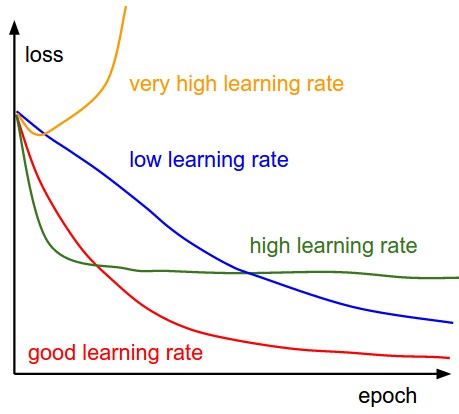
\includegraphics[width=6cm]{img/learning_rates_comparison}
	\caption{Visualization of the development of a loss function when using different learning rates.\protect\footnotemark}
	\label{fundamentals:figures:learning_rates}
\end{figure}
\footnotetext{http://cs231n.github.io/assets/nn3/learningrates.jpeg}
